\documentclass[a4paper, 12pt]{article}
% packages
\usepackage{amssymb}
\usepackage[fleqn]{mathtools}
\usepackage{tikz}
\usepackage{enumerate}
\usepackage{bussproofs}
\usepackage{xcolor}
\usepackage[margin=1.3cm]{geometry}
\usepackage{logicproof}
\usepackage{diagbox}
\usepackage{listings}
\usepackage{graphicx}
\usepackage{lstautogobble}
\usepackage{hyperref}
\usepackage{multirow}
\usepackage{stmaryrd}
\usetikzlibrary{arrows, shapes.gates.logic.US, circuits.logic.US, calc, automata, positioning}

% shorthand for verbatim
\catcode`~=\active
\def~#1~{\texttt{#1}}

% code listing
\lstdefinestyle{main}{
    numberstyle=\tiny,
    breaklines=true,
    showspaces=false,
    showstringspaces=false,
    tabsize=2,
    numbers=left,
    basicstyle=\ttfamily,
    columns=fixed,
    fontadjust=true,
    basewidth=0.5em,
    autogobble,
    xleftmargin=3.0ex,
    mathescape=true
}
\newcommand{\dollar}{\mbox{\textdollar}} %
\lstset{style=main}

% augmented matrix
\makeatletter
\renewcommand*\env@matrix[1][*\c@MaxMatrixCols c]{%
\hskip -\arraycolsep
\let\@ifnextchar\new@ifnextchar
\array{#1}}
\makeatother

% ceiling / floor
\DeclarePairedDelimiter{\ceil}{\lceil}{\rceil}
\DeclarePairedDelimiter{\floor}{\lfloor}{\rfloor}

% custom commands
\newcommand{\indefint}[2]{\int #1 \, \mathrm{d}#2}
\newcommand{\defint}[4]{\int_{#1}^{#2} #3 \, \mathrm{d}#4}
\newcommand{\dif}[2]{\frac{\mathrm{d}#1}{\mathrm{d}#2}}
\newcommand{\limit}[2]{\displaystyle{\lim_{#1 \to #2}}}
\newcommand{\summation}[3]{\sum\limits_{#1}^{#2} #3}
\newcommand{\intbracket}[3]{\left[#3\right]_{#1}^{#2}}
\newcommand{\ulsmash}[1]{\underline{\smash{#1}}}

\newcommand{\powerset}[0]{\wp}
\renewcommand{\emptyset}[0]{\varnothing}
\newcommand{\la}[0]{\langle}
\newcommand{\ra}[0]{\rangle}

\newcommand{\unaryproof}[2]{\AxiomC{#1} \UnaryInfC{#2} \DisplayProof}
\newcommand{\binaryproof}[3]{\AxiomC{#1} \AxiomC{#2} \BinaryInfC{#3} \DisplayProof}
\newcommand{\trinaryproof}[4]{\AxiomC{#1} \AxiomC{#2} \AxiomC{#3} \TrinaryInfC{#4} \DisplayProof}

% no indent
\setlength\parindent{0pt}
\setlength\itemsep{0em}

% reasoning proofs
\usepackage{ltablex}
\usepackage{environ}
\keepXColumns
\NewEnviron{reasoning}{
    \begin{tabularx}{\textwidth}{rlX}
        \BODY
    \end{tabularx}
}
\newcommand{\proofline}[3]{$(#1)$ & $#2$ & \hfill #3 \smallskip \\}
\newcommand{\proofarbitrary}[1]{& take arbitrary $#1$ \smallskip \\}
\newcommand{\prooftext}[1]{\multicolumn{3}{l}{#1} \smallskip \\}
\newcommand{\proofmath}[3]{$#1$ & = $#2$ & \hfill #3 \smallskip \\}
\newcommand{\prooftherefore}[1]{& $\therefore #1$ \smallskip \\}
\newcommand{\proofbc}[0]{\prooftext{\textbf{Base Case}}}
\newcommand{\proofis}[0]{\prooftext{\textbf{Inductive Step}}}

% reasoning er diagrams
\newcommand{\nattribute}[4]{
    \node[draw, state, inner sep=0cm, minimum size=0.2cm, label=#3:{#4}] (#1) at (#2) {};
}
\newcommand{\mattribute}[4]{
    \node[draw, state, accepting, inner sep=0cm, minimum size=0.2cm, label=#3:{#4}] (#1) at (#2) {};
}
\newcommand{\dattribute}[4]{
    \node[draw, state, dashed, inner sep=0cm, minimum size=0.2cm, label=#3:{#4}] (#1) at (#2) {};
}
\newcommand{\entity}[3]{
    \node[] (#1-c) at (#2) {#3};
    \node[inner sep=0cm] (#1-l) at ($(#1-c) + (-1, 0)$) {};
    \node[inner sep=0cm] (#1-r) at ($(#1-c) + (1, 0)$) {};
    \node[inner sep=0cm] (#1-u) at ($(#1-c) + (0, 0.5)$) {};
    \node[inner sep=0cm] (#1-d) at ($(#1-c) + (0, -0.5)$) {};
    \draw
    ($(#1-c) + (-1, 0.5)$) -- ($(#1-c) + (1, 0.5)$) -- ($(#1-c) + (1, -0.5)$) -- ($(#1-c) + (-1, -0.5)$) -- cycle;
}
\newcommand{\relationship}[3]{
    \node[] (#1-c) at (#2) {#3};
    \node[inner sep=0cm] (#1-l) at ($(#1-c) + (-1, 0)$) {};
    \node[inner sep=0cm] (#1-r) at ($(#1-c) + (1, 0)$) {};
    \node[inner sep=0cm] (#1-u) at ($(#1-c) + (0, 1)$) {};
    \node[inner sep=0cm] (#1-d) at ($(#1-c) + (0, -1)$) {};
    \draw
    ($(#1-c) + (-1, 0)$) -- ($(#1-c) + (0, 1)$) -- ($(#1-c) + (1, 0)$) -- ($(#1-c) + (0, -1)$) -- cycle;
}

% actual document
\begin{document}
    \section*{CO142 - Discrete Structures}
        \subsection*{Prelude}
            The content discussed here is part of CO142 - Discrete Structures (Computing MEng); taught by Steffen van Bakel, in Imperial College London during the academic year 2018/19. The notes are written for my personal use, and have no guarantee of being correct (although I hope it is, for my own sake). This should be used in conjunction with the (extremely detailed) notes.
        \subsection*{9th October 2018}
            \subsubsection*{Recommended Books}
                \begin{itemize}
                    \itemsep0em
                    \item K.H. Rosen. \textit{Discrete Mathematics and its Applications}
                    \item J.L. Gersting. \textit{Mathematical Structures for Computer Science}
                    \item J.K. Truss. \textit{Discrete Mathematics for Computer Science}
                    \item R. Johsonbaugh. \textit{Discrete Mathematics}
                    \item C. Schumacher. \textit{Fundamental Notions of Abstract Mathematics}
                \end{itemize}
                However, these books don't cover the same content. Learn his notation.
            \subsubsection*{Logical Formula, and Notation}
                This notation will be shared with \textbf{CO140}.
                \begin{itemize}
                    \itemsep0em
                    \item $A \land B$ \hfill $A$ and $B$ both hold
                    \item $A \lor B$ \hfill $A$ or $B$ holds (or both)
                    \item $\neg A$ \hfill $A$ does not hold
                    \item $A \Rightarrow B$ \hfill if $A$ holds, then so does $B$
                    \item $A \Leftrightarrow B$ \hfill $A$ holds if and only if $B$ holds
                    \item $\forall x (A)$ \hfill the predicate $A$ holds for all $x$
                    \item $\exists x (A)$ \hfill the predicate $A$ holds for some $x$
                    \item $a \in A$ \hfill the object $a$ is in the set $A$ ($a$ is an element of     \item $A$)
                    \item $a \notin A$ \hfill the object $a$ is not in the set $A$
                    \item $=_A$ \hfill tests whether two elements of $A$ are the same
                \end{itemize}
            \subsubsection*{Sets}
                Sets are like data types in Haskell: Haskell data type declaration;
                \begin{itemize}
                    \itemsep0em
                    \item \texttt{data Bool = False | True}
                    \item \texttt{\{false, true\}} \hfill set of boolean values
                    \item \texttt{[true, false, true, false]} \hfill list of boolean values
                    \item \texttt{\{false, true\} = \{true, false\}} \hfill set equality (note that order doesn't matter)
                \end{itemize}
                A set is a collection of objects from a pool of objects. Each object is an \textit{element}, or a \textit{member} of the set. A set \textit{contains} its elements. Sets can be defined in the following ways;
                \begin{itemize}
                    \itemsep0em
                    \item $\{a_1, ..., a_2\}$ \hfill as a collection of $n$ distinct elements
                    \item $\{x \in A \mid P(x)\}$ \hfill for all the elements in $A$, where $P$ holds
                    \item $\{x \mid P(x)\}$ \hfill for all elements, where $P$ holds (dangerous - Russel's paradox)
                \end{itemize}
            \subsubsection*{Use of "triangleq"}
                The use of $\triangleq$ is for "is defined by". Hence the empty set, $\varnothing \triangleq \{\}$. The difference between $\triangleq$ and $=$, is that the former cannot be proven, it is fact, whereas the latter takes work to prove.
            \subsubsection*{Russel's paradox}
                Not everything we write as $\{x \mid P(x)\}$ is automatically a set. Assume $R = \{X \mid X \notin X\}$ is a set, the set of all sets which don't contain themselves. As $R$ is a set, then $R \in R$, or $R \notin R$ (law of excluded middle), and thus we can do a case by case analysis.
                \begin{itemize}
                    \itemsep0em
                    \item Assume $R \in R$. By the definition of $R$, it then follows that $R \notin R$ (if $R \in R$, then it doesn't satisfy the definition of $R$) - which is a contradiction.
                    \item Assume $R \notin R$. It then follows that $R \in R$, as it follows the definition of $R$, hence it is another contradiction.
                \end{itemize}
                As both assumptions lead to contradictions, it's possible to write sets which aren't defined. We should only select from a set that we know is defined; $\{x \in A \mid P(x)\}$ - where $A$ is a well-defined set.
        \subsection*{12th October 2018}
            \subsubsection*{Set Comparisons}
                We can define a set $A$, as being a subset of another set $B$ if every element in $A$ is an element in $B$. This can be formally written as; $A \subseteq B \triangleq \forall x \in A (x \in B)$. Note that we can also say $\forall x (x \in A \Rightarrow x \in B)$, and the two hold the same meaning. It's important to clarify in the latter that we're not the domain of $x$, an we assume there is a universe of possible objects which forms a set. We're also able to define a strict subset such that $A \subset B \triangleq A \subseteq B \land A \neq B$.
                \medskip

                We can say that any set is a trivial subset of itself, as we'd have $x \in A \Rightarrow x \in A$, which always evaluates to true, from propositional logic. Another trivial example is that $\emptyset$, the empty set, is a subset of every set. Using the second definition of subset, we can say that as $x \in \emptyset$ is false, by definition, and anything follows from falsity, whereas in the first definition we argue that all (0) elements of $\emptyset$ are in some other set.
                \medskip

                We can also define set equality as $A = B \triangleq A \subseteq B \land B \subseteq A$. However, we can also consider the set composition notation for a set, such that $A = \{x \in C \mid P(x)\}$, and $B = \{x \in C \mid Q(x)\}$. If we're able to prove that $\forall x (P(x) \Leftrightarrow Q(x))$, it follos that $A = B$. This method can be quite powerful if we're familiar with logic, and equivalences. We can justify this by saying that $y \in A \Rightarrow P(y) \Rightarrow Q(y) \Rightarrow y \in B$, and also in the other direcion; $y \in B \Rightarrow Q(y) \Rightarrow P(y) \Rightarrow y \in A$. This however requires both sets to be constructed on top of some known set $C$.
            \subsubsection*{Set Composition}
                \begin{itemize}
                    \itemsep0em
                    \item $A \cup B \triangleq \{x \mid x \in A \lor x \in B\}$ \hfill set union
                    \item $A \cap B \triangleq \{x \in A \mid x \in B\}$ \hfill set intersection
                    \item $A \backslash B$ (or $A - B$) $\triangleq \{x \in A \mid x \notin B\}$ \hfill set difference
                    \item $A \triangle B \triangleq (A \backslash B) \cup (B \backslash A)$ \hfill symmetric set difference))
                    \item $A \cap B = \emptyset$ \hfill disjoint set
                \end{itemize}
            \subsubsection*{A Note on Proofs}
                Instead of writing out the formal definition, where we may lose the intuition, using a natural language (direct) proof is acceptable in this course.
                \medskip

                Consider the following proof; $A \subseteq B$, and $B \subseteq C$, then show $A \subseteq C$. Here, we want to show that any element of $A$, is also an element of $C$. We can approach this intuitively by taking an arbitrary $a \in A$. By the the first assumption, we can say $a \in B$. Then, by the second assumption, $a \in C$. However, we've taken an arbitrary $a$, therefore this follows $\forall a \in A (a \in C)$, therefore $A \subseteq C$.
                \medskip

                The crucial part of the aforementioned proof is the use of some \textbf{arbitrary} value. If we were to do a proof on the natural numbers, to show $\forall n \in \mathbb{N} [\text{even}(n)]$, and we proved even(2), it wouldn't prove it for all natural numbers.
                \medskip

                We also want to aim for a direct proof, instead of a proof by contradiction, since we will often do the following; assume $\neg A$, then we somehow get $A$, which causes a contradiction ($\lightning$), and therefore $A$. However, we still did all the work to prove $A$.
                \medskip

                Consider the proof to show that $C \cap D = D \cap C$. Let us first take some arbitary $x \in (C \cap D)$. By definition of union, we know that $x \in C$, and $x \in D$. Therefore, it also fits the predicate for $(D \cap C)$. As such, $C \cap D \subseteq D \cap C$. To prove the other direction is trivial, and almost identical to this direction. Since we've proved both directions of $\subseteq$, we can conclude equality.
                \medskip

                Prove that $A = (A \backslash B) \cup (A \cap B)$. I took the approach where we use predicate logic, since I assumed it would be much easier than proving both directions of $\subseteq$ (turns out that the proof is very similar as proving one direction, is proving the other). In order to keep my proof cleaner, let $a \triangleq x \in A$, $b \triangleq x \in B$, and the negations $\neg a \triangleq x \notin A$ (and similar for $b$). Let us now define $A = \{x \mid P(x)\}$, where $P(x) = a$, and $B = \{x \mid Q(x)\}$, where $Q(x) = (a \land \neg b) \lor (a \land b)$ - by definitions of set difference, union, and intersection. Since this proves equivalence between the two predicates, we can therefore prove that the sets are equal.
                \begin{reasoning}
                    \proofmath{Q(x)}{(a \land \neg b) \lor (a \land b)}{}
                    \proofmath{}{[(a \land \neg b) \lor a] \land [(a \land \neg b) \lor b]}{$(B \land C) \lor A \equiv (A \lor B) \land (A \lor C)$}
                    \proofmath{}{(a \lor a) \land (a \lor \neg b) \land (a \lor b) \lor (b \lor \neg b)}{$(B \land C) \lor A \equiv (A \lor B) \land (A \lor C)$ (twice)}
                    \proofmath{}{a \land (a \lor \neg b) \land (a \lor b)}{$A \lor A \equiv A$, $A \lor \neg A \equiv \top$, and $A \land \top \equiv A$}
                    \proofmath{}{a}{$A \land (A \lor B) \equiv A$ (twice)}
                    \proofmath{}{P(x)}{}
                \end{reasoning}
        \subsection*{16th October 2018}
            \subsubsection*{A Note on the Use of Venn Diagrams}
                While we can use a Venn diagram to aid in constructing a counter example, the diagram itself is not a counter example. We're also quite limited in the possible uses, as a diagram (in 2d) consisting of $\geq 4$ sets doesn't represent all the possible combinations of sets.
            \subsubsection*{Operator Properties}
                Similar to \textbf{CO140}, we have some properties which can be used on arbitrary sets. Note that these are not axioms, and therefore we are able to prove them.
                \begin{itemize}
                    \itemsep0em
                    \item $A \cup A = A$ \hfill indempotence
                    \item $A \cap A = A$ \hfill indempotence
                    \item $A \cup B  = B \cup A$ \hfill commutativity
                    \item $A \cap B  = B \cap A$ \hfill commutativity
                    \item $A \triangle B  = B \triangle A$ \hfill commutativity
                    \item $A \cup (B \cup C) = (A \cup B) \cup C$ \hfill associativity
                    \item $A \cap (B \cap C) = (A \cap B) \cap C$ \hfill associativity
                    \item $A \cup \emptyset = A$ \hfill empty set
                    \item $A \cap \emptyset = \emptyset$ \hfill empty set
                    \item $A \triangle A = \emptyset$ \hfill empty set
                    \item $A \cup (B \cap C) = (A \cup B) \cap (A \cup C)$ \hfill distributivity
                    \item $A \cap (B \cup C) = (A \cap B) \cup (A \cap C)$ \hfill distributivity
                    \item $A \cup (A \cap B) = A$ \hfill absorption
                    \item $A \cap (A \cup B) = A$ \hfill absorption
                \end{itemize}
                Note that we are able to use the properties of logical connectives to aid us in our proofs, since those are fairly easy to prove with truth tables, as they have a finite number of configurations. For example, the proof of indempotence inherently uses the property $p \land p \equiv p$, and the same for $\lor$.
            \subsubsection*{Cardinality}
                With some finite set $A$, we can say that the cardinality, $|A|$ is the number of distinct elements in $A$. Given two finite sets, we can then say that $|A \cup B| = |A| + |B| - |A \cap B|$. With the following set properties (and that for two disjoint finite sets, $|A \cup B| = |A| + |B|$), and knowing the RHSs are disjoint unions;
                \begin{reasoning}
                    \proofmath{A}{(A \backslash B) \cup (A \cap B)}{}
                    \proofmath{B}{(B \backslash A) \cup (A \cap B)}{}
                    \proofmath{A \cup B}{(A \backslash B) \cup (A \cap B) \cup (B \backslash A)}{}
                    \proofmath{|A|}{|A \backslash B| + |A \cap B|}{}
                    \proofmath{|B|}{|B \backslash A| + |A \cap B|}{}
                    \proofmath{|A \cup B|}{|A \backslash B| + |A \cap B| + |B \backslash A|}{}
                    \proofmath{}{|A| - |A \cap B| + |A \cap B| + |B| - |A \cap B|}{}
                    \proofmath{}{|A| + |B| - |A \cap B|}{}
                \end{reasoning}
        \subsection*{19th October 2018}
            \subsubsection*{Powerset}
                Let us define the powerset of $A$, as $\powerset A \triangleq \{x \mid x \subseteq A\}$. It's therefore important to note that $\powerset \emptyset = \{\emptyset\}$, hence the powerset of the empty set has size 1. We can prove that $|\powerset X| = 2^n$, for some set $X$, where $|X| = n$. This can be done (fairly) easily with mathematical induction, over natural numbers. Another approach it is to consider that each item in some arbitrary set, $A = \{a_1, a_2, ... a_n\}$, can either be in the powerset or not. Therefore, we can represet each subset of $A$ as some $n$-bit binary number. Therefore, we can have a $2^n$ possible combinations, hence the size of $|\powerset A| = 2^n$
            \subsubsection*{Products}
                Let us define some \textbf{ordered} pair as $\langle a, b \rangle$, such that generally $\la a, b \ra \neq \la b, a \ra$.
                \medskip

                Let there be some arbitrary sets $A$, and $B$. We can then define the cartsian product as follows; $A \times B \triangleq \{\la a, b \ra \mid a \in A \land b \in B\}$. Since we'll often deal with binary relations, we use the shorthand $A^2 = A \times A$. We can define equality on ordered pairs as $\forall a, b, c, d [\la a, b \ra =_{A \times B} \la c, d \ra \triangleq a =_A c \land b =_B d]$. Note that in general, $\times$ is not a commutative operation.
                \medskip

                Suppose that there are two finite sets $A = \{a_1, a_2, ..., a_n\}$, and $B = \{b_1, b_2, ..., b_m\}$, with sizes $n$, and $m$ respectively - then it follows that $|A \times B| = |A| \cdot |B|$. We can justify this by constructing such a matrix $R$, of dimension $(A \times B)^{n,m}$ - thus having $n \cdot m$ elements;
                \begin{center}
                    $R = \begin{matrix}
                        \la a_1, b_1 \ra & \la a_1, b_2 \ra & \cdots & \la a_1, b_m \ra \\
                        \la a_2, b_1 \ra & \la a_2, b_2 \ra & \cdots & \la a_2, b_m \ra \\
                        \vdots & \vdots & \ddots & \vdots \\
                        \la a_n, b_1 \ra & \la a_1, b_2 \ra & \cdots & \la a_n, b_m \ra \\
                    \end{matrix}$
                \end{center}
                We can also have an $n$-ary product, to construct an $n$-tuple $\la a_1, a_2, ..., a_n \ra$, when $n \geq 1$. Let there be some arbitrary sets, $A_1, A_2, ..., A_n$.
                \smallskip

                This is written as $A_1 \times ... \times A_n = \prod\limits_{i = 1}^n A_i$, and is defined as $\{\la a_1, a_2, ..., a_n \ra \mid \forall i \in [1, n] [a_i \in A_i]\}$.
            \subsubsection*{Partitions}
                Given some set $S$, we can define a \textbf{partition} of $S$ to be a family of subsets $\{A_1, A_2, ..., A_n\}$ such that;
                \begin{itemize}
                    \itemsep0em
                    \item none of them are empty (therefore $\forall i \in [1, n] [A_i \neq \emptyset]$)
                    \item the subsets cover $S$ (therefore $S = \bigcup\limits_{i = 1}^n A_i$)
                    \item they are pairwise disjoint (therefore $\forall i, j \in [1, n] [i \neq j \Rightarrow A_i \cup A_j = \emptyset]$)
                \end{itemize}
                A partition of $S$ is a set of non-empty subsets that are pairwise disjoint, and cover $S$.
            \subsubsection*{Pigeonhole Principle}
                Given a set $S$ of size $n$, partitioned into $k$ sets such that $0 < k < n$, then at least one of the subsets must have at least 2 elements. We can prove this by contradiction (one of the few times we actually do this, in DS). Assume that there are $k$ subsets, each of size 1 (therefore $\forall i \in [1, k] [|A_k| = 1]$). By definition of a partion, we can form a cover of $S$, therefore (the last 2 steps are justfied by the requirement of a partiion being pairwise disjoint);
                \smallskip

                $n = |S| = |\bigcup\limits_{i = 1}^k A_i| = \summation{i = 1}{k}{|A_i|} = \summation{i = 1}{k}{1} = k$
                \smallskip

                However, given the bounding condition $k < n$, there is no way that $k = n$, and the only assumption is that we made $k$ sets of size 1.
            \subsubsection*{Representing Relations}
                We define a relation between two sets $A$, and $B$ (from $A$ to $B$), as a subset of $A \times B$, such that $R \subseteq A \times B$. If we say that $R \subseteq A \times B$, it means that it has type $A \times B$. However, if $R \subseteq A^2$, it is a \textbf{binary} relation on $A$. Instead of writing $\la a, b \ra \in \mathbb{R}$, we will often shorten it to $a\ R\ b$.
                \medskip

                A relation does not have to be meaningful; for a set of size $n = 2$, let it be $A = \{a, b\}$, it can have 16 $(2^{n^2})$ possible binary relations. For any set $A$, the possible binary relations can be generated by taking $\powerset A^2$. A predicate over $A$ is a 1-ary relation, which is just a subset of $A$. We also can say something along the lines of $\{\la x, y, z \ra \in \mathbb{R}^3 \mid x^2 + y^2 + z^2 = 1\}$, as a ternary relation on the reals which covers the surface of a unit sphere at the origin.
                \medskip

                Generally, writing out all pairs can become tedious, therefore there are numerous other ways of representing it. We can construct a diagram (a bipartite graph) for the following relation $A = \{a_1, a_1\}$, $B = \{b_1, b_2, b_3\}$, and $R = \{\la a_1, b_1 \ra, \la a_2, b_1 \ra, \la a_2, b_2 \ra\}$;
                \begin{center}
                    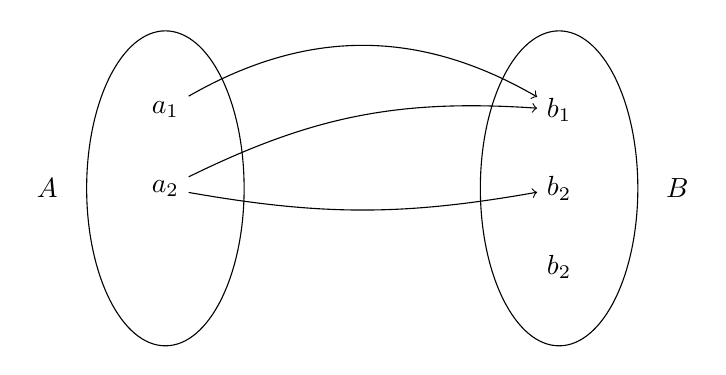
\begin{tikzpicture}
                        \node[] () at (-1.5, 0) {$A$};
                        \node[] () at (6.5, 0) {$B$};
                        \node[] (a1) at (0, 1) {$a_1$};
                        \node[] (a2) at (0, 0) {$a_2$};
                        \node[] (b1) at (5, 1) {$b_1$};
                        \node[] (b2) at (5, 0) {$b_2$};
                        \node[] (b3) at (5, -1) {$b_2$};
                        \draw
                        (0,0) ellipse (1 and 2)
                        (5,0) ellipse (1 and 2)
                        (a1) edge[bend left=30, ->] (b1)
                        (a2) edge[bend left=15, ->] (b1)
                        (a2) edge[bend right=10, ->] (b2);
                    \end{tikzpicture}
                \end{center}
                However, we might also want to represent a binary relation in a similar way, in which case we can draw a regular directed graph. Here we have $A = \{a_1, a_2, a_3, a_4\}$, and $R = \{\la a_1, a_2 \ra, \la a_2, a_1 \ra, \la a_3, a_2 \ra, \la a_3, a_3 \ra\}$;
                \begin{center}
                    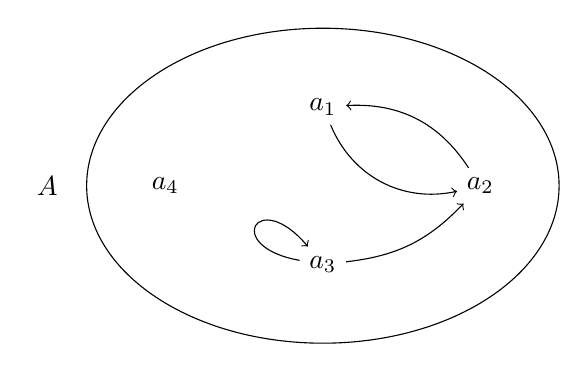
\begin{tikzpicture}
                        \node[] () at (-3.5, 0) {$A$};
                        \node[] (a1) at (0, 1) {$a_1$};
                        \node[] (a2) at (2, 0) {$a_2$};
                        \node[] (a3) at (0, -1) {$a_3$};
                        \node[] (a4) at (-2, 0) {$a_4$};
                        \draw
                        (0, 0) ellipse (3 and 2)
                        (a3) edge[loop, ->, out=170, in=130, distance=1cm] (a3)
                        (a3) edge[bend right=20, ->] (a2)
                        (a2) edge[bend right=30, ->] (a1)
                        (a1) edge[bend right=40, ->] (a2);
                    \end{tikzpicture}
                \end{center}
                It can also be represented as a matrix, such that we have
                \begin{equation*}
                    M_{i,j} =
                    \begin{cases}
                        \text{True} & \text{if } a_i\ R\ b_j \\
                        \text{False} & \text{otherwise}
                    \end{cases}
                \end{equation*}
            \subsubsection*{Constructing Relations}
                Just like in sets, we can construct relations quite easily. Except, we now have a known set in they exist in (by the subset definition), hence (these examples use $R, S \subseteq A \times B$, and $T \subseteq B \times C$);
                \begin{itemize}
                    \itemsep0em
                    \item $R \cup S \triangleq \{\la a, b \ra \in A \times B \mid \la a, b \ra \in A \lor \la a, b \ra \in B\}$ \hfill relation union
                    \item $R \cap S \triangleq \{\la a, b \ra \in A \times B \mid \la a, b \ra \in A \land \la a, b \ra \in B\}$ \hfill relation intersection
                    \item $\overline{R} \triangleq \{\la a, b \ra \in A \times B \mid \la a, b \ra \notin A\}$ \hfill relation complement
                    \item $R^{-1} \triangleq \{\la b, a \ra \in B \times A \mid a\ R\ b\}$ \hfill inverse relation
                    \item $\text{id}_A \triangleq \{\la x, y \ra \in A^2 \mid x =_A y\}$ \hfill identity relation
                    \item $R \circ T \triangleq \{\la a, c \ra \in A \times C \mid \exists b \in B [a\ R\ b \land b\ T\ c]\}$ \hfill relation composition
                        \subitem this is only defined when the types are matching
                        \subitem we can define grandparentof $\triangleq$ parentof $\circ$ parentof
                        \subitem therefore $x \text{ gpo } y \triangleq \exists z (x \text{ po } z \land z \text{ po } y)$
                \end{itemize}
        \subsection*{23rd October 2018}
            To be honest, this lecture was basically just a tutorial. Some solutions are listed here;
            \subsubsection*{Associativity of $\circ$}
                For arbitrary relations, $R \subseteq A \times B$, $S \subseteq B \times C$, and $T \subseteq C \times D$, show that $R \circ (S \circ T) = (R \circ S) \circ T$
                \medskip

                Take some arbitrary $\la x, y \ra \in R \circ (S \circ T)$;
                \begin{align*}
                    x\ R \circ (S \circ T)\ y \triangleq &\ \exists z [x\ R\ z \land z\ (S \circ T)\ y] \\
                    \triangleq &\ \exists z [x\ R\ z \land \exists w [z\ S\ w \land w\ T\ y]] \\
                    \Leftrightarrow &\ \exists w, z [x\ R\ z \land z\ S\ w \land w\ T\ y] \\
                    \Leftrightarrow &\ \exists w [x\ (R \circ S)\ w \land w\ T\ y] \\
                    \triangleq &\ x\ (R \circ S) \circ T\ y
                \end{align*}
                The key point to take from this proof is how we can use our knowledge of propositional logic, and apply it to sets. Since propositional logic is far easier to prove than an arbitrary set, we can reduce the work we do significantly.
            \subsubsection*{Subsets of Inverse Relations}
                Given two binary relations $R, S \subseteq A^2$, prove that $R \subseteq S \Rightarrow R^{-1} \subseteq S^{-1}$
                \medskip

                Take some arbitrary $\la y, x \ra \in R^{-1}$. In order to show the RHS, we want to show that this is also in $S^{-1}$. Let us also make the assumption (the LHS) that $R \subseteq S$, such that $k \in R \Rightarrow k \in S$, where $k$ is any tuple. As we have some $\la y, x \ra \in R^{-1}$, it follows that there is a corresponding $\la x, y \ra \in R$. Because of our assumption, we can say that $\la x, y \ra \in S$, and therfore $\la y, x \ra \in S^{-1}$. Therefore, any arbitrary element of $R^{-1}$ is also in $S^{-1}$, hence $R^{-1} \subseteq S^{-1}$ (given our assumption holds) - so $R \subseteq S \Rightarrow R^{-1} \subseteq S^{-1}$.
        \subsection*{26th October 2018}
            The first part is just some stuff about how you should be doing proofs in natural language, as mathematics (and symbols) is just formalised human thinking. This then goes into (basically) natural deduction - so check \textbf{CO140} for techniques you can apply in proofs. Once again, we went through more questions in this lecture.
            \subsubsection*{Relation Properties}
                Let there be $R \subseteq A^2$, such that $R$ is a binary relation on $A$;
                \begin{itemize}
                    \itemsep0em
                    \item $R$ is reflexive $\triangleq \forall x \in A [\la x, x \ra \in R]$
                        \subitem $\Leftrightarrow \text{id}_A \subseteq R$
                    \item $R$ is symmetric $\triangleq \forall x, y \in A [\la x, y \ra \in A \Rightarrow \la y, x \ra \in R]$
                        \subitem $\Leftrightarrow R = R^{-1}$
                    \item $R$ is transitive $\triangleq \forall x, z \in A [\exists y \in A [\la x, y \ra \in R \land \la y, z \ra \in R] \Rightarrow \la x, z \ra \in R]$
                        \subitem $\Leftrightarrow R \circ R \subseteq R$
                    \item $R$ is an equivalence relation if it is reflexive, symmetric, and transitive
                \end{itemize}
                We consider something to be an equivalence if it has a weak equality, such that $a\ R\ b$ means that $a$ is indistinguishable from $b$ in some sense. We can write this as $a \sim_R b$.
        \subsection*{30th October 2018}
            \subsubsection*{Equivlence Classes}
                Given $n \neq 0$, and $n \in \mathbb{N}$, the binary relation $R_n$ on $\mathbb{Z}$ is defined by $a\ R_n\ b$ when $n$ divides into $(b - a)$ is defined as; $R_n \triangleq \{\la a, b \ra \in \mathbb{Z}^2 \mid \exists q \in \mathbb{Z} [q \cdot n = (b - a)]\}$. This means that two numbers are in the same equivalence class given that they are an integer multiple of $n$ apart. As such, they have the same result under modulo $n$.
                \medskip

                Suppose we have some $R$, which is an equivalence relation on $A$. For any $a \in A$, we can define the equivalence class of $a$ with respect to $R$ as follows; $[a]_R \triangleq \{b \in A \mid a \sim_R b\}$. For brevity, we can omit the $_R$ when it's clear what equivalence relation we're referring to from the context. The set of equivalnce classes is referred to as the \textbf{quotient set}; $\frac{A}{R}$; therefore with the example above, the set $\frac{\mathbb{Z}}{R_n}$ is the quotient set which represents integers which have modulo $n$.
                \medskip

                Let us propose that the set of all equivalence classes, $\{[a] \mid a \in A\}$, forms a partiion of $A$. This means that the equivalence classes aren't empty, they form a cover of $A$, and that they are pairwise disjoint.
                \medskip

                We need to first show that no equivalence class is empty. First, let's take some arbitrary $x \in A$. By the reflexive nature of equivalences, we know that $x \sim_R x$, hence $x \in [x]$. As we took an arbitrary element of $A$, it's satisfied for all $A$, therefore none of the equivalnce classes are empty.
                \medskip

                Next we need to prove that it forms a cover of $A$, such that $A = \bigcup\limits_{a \in A}[a]$; done by proving that $A \subseteq \bigcup\limits_{a \in A}[a]$, and also $\bigcup\limits_{a \in A}[a] \subseteq A$.
                \smallskip

                Doing the former, let us take some arbitrary $x \in A$. Now, it follows that it's in its own equivalence class $[x]$, under the same justification we gave for the first part of the proof ($x \sim_R x$ by reflexivity). Trivially, we can say that $[x] \subseteq \bigcup\limits_{a \in A}[a]$. Hence $x \in \bigcup\limits_{a \in A}[a]$, and as we took arbitrary $x$; $A \subseteq \bigcup\limits_{a \in A}[a]$.
                \medskip

                To prove the other direction, take some arbitrary equivalence class $[x] \in \bigcup\limits_{a \in A}[a]$, and arbitrary $y \in [x]$. This then means we've taken arbitrary $y \in \bigcup\limits_{a \in A}[a]$.
                \smallskip

                By our definition of an equivalence class, for $y \in [x]$, it must therefore mean $x \sim_R y$, and also that $y \in A$. Hence we get $\bigcup\limits_{a \in A}[a] \subseteq A$. As we have both directions of $\subseteq$, we conclude the two sets are equal.
                \medskip

                The last one can be done by proving two equivalence classes are equal, if they aren't pairwise disjoint. Suppose two arbitrary classes in the set of equivalnce classes aren't pairwise disjoint, such that $[x] \cap [y] \neq \emptyset$. Therefore, this means that $w \in ([x] \cap [y])$, by definition of set union, we can then say that $w \in [x]$, and also $w \in [y]$. This then leads to $x \sim_R w$, and also $y \sim_R w$, by definition. However, by symmetry, we can rewrite the former as $w \sim_R x$. To establish equality, we need to show that they are subsets of each other (will only do one, since it's trivial to do the other way around). Take some arbitrary $v \in [x]$, then it follows that $x \sim_R v$. By transitivity, we can now say $w \sim_R v$, and therefore also $y \sim_R v$. It then follows that $v \in [y]$. As we took arbitrary $v \in [x]$, it follows that $[x] \subseteq [y]$. Hence the only way two items aren't disjoint in a set of equivalence classes, is when they are equal. Thus, the family of equivalence classes is pairwise disjoint, and is a partion of $A$.

\end{document}